\documentclass[class=article]{standalone}
%----------------------------Preamble-------------------------------%
\usepackage{tikz}                       % Drawing/graphing tools.
\usetikzlibrary{arrows.meta}            % Latex and Stealth arrows.
%--------------------------Main Document----------------------------%
\begin{document}
    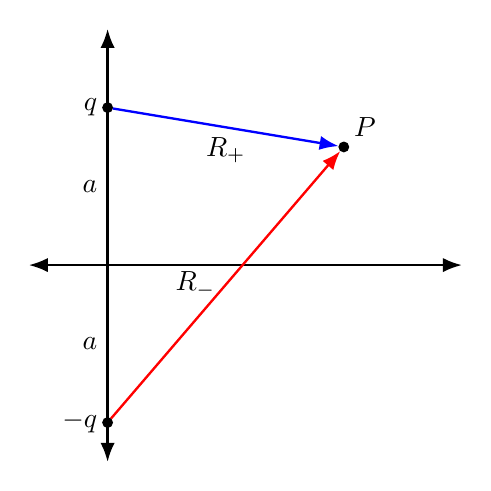
\begin{tikzpicture}[%
        line width=0.3mm,
        >={Latex},
    ]
        \begin{scope}[%
            every node/.style={
                circle,
                fill=black,
                draw=black,
                inner sep=0pt,
                minimum size=3pt
            }
        ]
            \node (q) at (0,2) {};
            \node (-q) at (0,-2) {};
            \node (P) at (3,1.5) {};
        \end{scope}
        \node at (q) [left] {$q$};
        \node at (-q) [left] {$-q$};
        \node at (P) [above right] {$P$};
        \draw[<->] (0,-2.5) -- (0,3);
        \draw[<->] (-1,0) -- (4.5,0);
        \draw[->,draw=blue] (q) -- node [below] {$R_{+}$} (P);
        \draw[->,draw=red] (-q) -- node [left] {$R_{-}$} (P);

        \node at (0,1) [left] {$a$};
        \node at (0,-1) [left] {$a$};
    \end{tikzpicture}
\end{document}